\chapter{Methods}

In this chapter, onset annotation, onset detection evaluation, automatic rhythm assessment and its evaluation are explained. 

\section{Onset Annotations of Datasets}

\subsection{MusicCritic Dataset}\label{mc_annot}
Recordings are manually annotated by the author, using the Sound Annotation & Analysis Tool (see Appendix A for details) developed during the course of this work. This tool made the analysis of the sounds and comparison of algorithms easier. It can display many audio features from Essentia \cite{essentia} library and predictions of multiple onset detection algorithms on its interactive plots.

Prior to the annotation session, two buttons are assigned to stamps "Onset" and "Crop". "Onset" stamp is used for onsets of single notes and chords. "Crop" is used at the beginning and end of the recordings to remove silenced or unrelated parts. Annotation is done by pressing the stamp on the keyboard and clicking on the plot. The annotator can start and stop playing recordings freely during the process. A moving cursor is aligned with the sound being played to show the location. The annotator wore headphones in a quiet environment. Both visual and aural cues are used in determining the onset locations.  

For a single note, the maximum location of the waveform is selected as the onset time. For a chord, the first perceivable note is aimed on the waveform. On each recording, the plot is zoomed to contain at most 4 onsets. When the visual cue is weak (e.g. a weak note is played when the previous note is not decayed yet), annotation is done after additional zoom and repeated listening.

\subsection{GuitarSet}
Onset annotations of GuitarSet are already available, but they are separate for each string. We deduce the onset locations of strings in a chord to a single location. Onset locations that are closer than 0.025 ms are grouped (e.g. 6 string chord may span up to 0.125 ms) and then their average is taken as the chord onset. Apart from taking the average, last onsets and first onsets are also tested in evaluations. The effect on overall scores is found to be negligible.

\section{Evaluation of Onset Detection Algorithms}

The mir\_eval \cite{raffel2014mir_eval} library is used for onset detection evaluation. The evaluation method is the same as the method used in MIREX evaluations. An onset is correctly detected if there is an onset prediction inside the tolerance window. The standard size of the tolerance window is 50 ms. If there are more than one prediction for the same true onset (called the doubled onsets), excess predictions are added to the false positive onsets. If there is one prediction for two onsets (called the merged onsets), excess true onsets are added to the false negative onsets.

TP: True Positive
FP: False Positive
TN: True Negative
FN: False Negative

Precision \(P = \frac{TP}{TP+FP}\)\\
Recall \(R = \frac{TP}{TP+FN}\)\\
F-score \(F = \frac{2\cdot P\cdot R}{P+R}\)\\

A set of onset detection algorithms (Complex \cite{bello2004use}, Complex Phase \cite{brossier2004fast}, Superflux \cite{bock2013maximum}, NINOS$^2$ \cite{mounir2016guitar},  HFC \cite{masri1996imroved}, RNNOnsetDetector \cite{eyben2010universal}, CNNOnsetDetector \cite{schluter2014improved}) are evaluated on GuitarSet with the standard tolerance window size of 50 ms (Table \ref{tab:GSothers}). The most promising algorithm (CNNOnsetDetector), together with MC-OnsetDetector and the algorithm developed in this work are evaluated on both GuitarSet and MusicCritic datasets. This time the evaluation is more detailed.

Nearly half of each dataset consist of chords. Chords' attack time may vary depending on the strumming speed of the player, and it may exceed the tolerance window size. There is no consensus on the onset location of a chord and algorithms may aim at different locations on the sound envelope. To make the evaluation fair, onset predictions are re-evaluated eleven times by shifting them, from -50 ms to +50 with 10 ms increments. The highest F-score among those evaluations is accepted as the score of the algorithm. 

\section{Automatic Rhythm Assessment}\label{assessmethod}

The automatic rhythm assessment algorithm consists of three parts: onset detection, processing (feature extraction), and prediction. In the processing part, features are created using the predicted onsets. Those features are then used to predict the grades. We keep the processing and prediction parts the same with the previous work  \cite{eremenko2020performance} and the evaluation as well, to measure the effect of different onset detection algorithms. The problem is that it is not clear how to process the onset locations for rhythm assessment. There are a few studies where onset locations are processed for rhythm assessment \cite{percival2008thesis} \cite{abesser2014automatic} \cite{wu2016towards} \cite{falcaoMast}, but they are evaluated on different datasets. Here we explain how the onsets are processed in this work. Our aim is to identify a minimal processing method that allows a fair comparison of the onset detection algorithms.

In the previous work, predictions were made by applying isotonic regression \cite{mair2009isotone} to processed onsets. In this work, we do the same. In the processing part, deviations of onset predictions from the metrical positions were taken. The metrical positions are aligned with a metronome that students can hear while playing. This method is not accurate when the chords are strummed. On strummed chords, beat location is not clearly defined. Players choose the beat location subjectively \cite{freire2018strumming}. Beat location is subjective also for the listeners \cite{hove2007sensorimotor}. This means that the difference between an onset prediction and the metronome beat is not enough to determine the timing of the chord. For this reason, a different method is used in this work. We argue that the time differences between onset predictions are better features than the differences between onsets predictions and metronome beats. For the following reasons: 

\begin{itemize}
  \item In a recording, the factors that affect the characteristics of a strummed chord (e.g. player, instrument, recording device and the environment) stays the same. It can be assumed that the characteristics of the strummed chords (or the single notes) in that recording are with each other, when compared to chords from different recordings.
  
  \item In a recording where the characteristics of strummed chords are consistent, it can be assumed that the locations of onset predictions of an algorithm are also going to be consistent.  
\end{itemize}

Perceived beat locations are also consistent for players \cite{freire2018strumming} and listeners \cite{hove2007sensorimotor}. If all of the consistencies in the assumptions were perfect, the time differences of onset predictions would be equal to the time differences of the listener's (and player's) beat locations (e.g. in Figure \ref{fig:devi}, differences between red lines are equal to the differences between green lines). If the consistencies are not perfect, the time differences are not equal but still correlated. So, the time difference of onset predictions represents the perceived beats better than the differences from the metronome beats, since the differences from the metronome beats are subjective. 

We normalize the time differences by their tempo, so the machine learning algorithm can be used effectively. Normally, we should take the deviations of time differences from the corresponding beat duration. Since the exercises in the MusicCritic dataset only contains quarter notes, we can use the deviations from the tempo directly. 

\begin{figure}
    \centering
    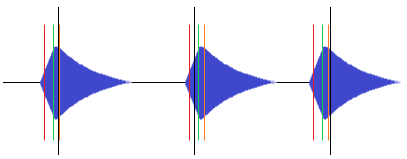
\includegraphics[width=\columnwidth]{methods/devi.png}
    \caption{A toy example of identical strummed chords. Timing of a strummed chord can only be understood when it is compared to other chords. Given three chords, the chord in the middle is played late. (Black line is metronome. Red, green and orange lines are onset predictions, listener's beat locations and student's beat locations, in any order.)}
    \label{fig:devi}
\end{figure}

In the prediction part, the isotonic regression is applied to onset difference deviations to predict the rhythm grades of the MusicCritic dataset.

